\documentclass[titlepage]{article}
\usepackage{babel}
\usepackage{amsmath}
\usepackage{amssymb}
\usepackage{amsthm}
\usepackage{tabto} %tabulator mit \tab
\usepackage{tikz}
\usetikzlibrary{automata, arrows.meta, positioning, shadows, shapes.geometric} % automaten zeichnen
\usepackage[utf8]{inputenc}
\pagestyle{plain}
\pagenumbering{arabic}
\renewcommand{\arraystretch}{1.3} %vertikaler abstand von tabellen
\usepackage[left=20mm, right=15mm, top=25mm, bottom=7mm, paper=a4paper]{geometry}

\renewcommand{\contentsname}{Inhaltsverzeichnis}
\renewcommand{\]}{\right]}
\renewcommand{\[}{\left[}
\renewcommand{\)}{\right)}
\renewcommand{\(}{\left(}
\renewcommand{\|}{\;|\;}
\newcommand{\n}{\newline}
\renewcommand{\l}{\linebreak}



\begin{document}\begingroup\let\clearpage\relax
	%header
	\begin{center}
	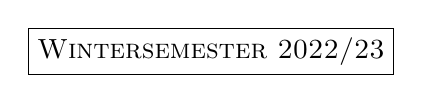
\begin{tikzpicture}
		\draw (0,0) node[draw, rectangle]{\textsc{Wintersemester 2022/23}};
	\end{tikzpicture}
	\hrulefill\\
	\begin{center}
		\LARGE\textsc{Automaten und Berechenbarkeit - Übung 04} \normalsize\\
	\end{center}
	\hrulefill
	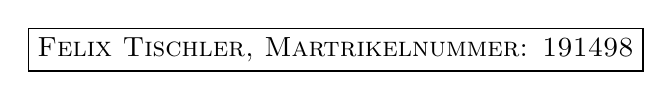
\begin{tikzpicture}
		\draw (0,0) node[draw, rectangle]{\textsc{Felix Tischler, Martrikelnummer: 191498}};
	\end{tikzpicture}
	\date{\today}
\end{center}
	
	%task one
	\section*{Aufgabe 1}
		Untersuchen Sie, ob die folgenden Sprachen regulär sind oder nicht:
		\subsection*{(a) $A=\{w\mid w\in\{a,b\}^*,\#_a(w)=2\#_b(w)\}$}
			\begin{proof}[Beweis]
	\begin{math}
		Ann:\;A\in REG\Rightarrow\;es\;gilt\;PL\Leftrightarrow\;Sei\;k\;Pumpingzahl:
	\end{math}
	\begin{align*}
		&Wähle\;x=\underbrace{a^{j_1}}_u\underbrace{a^{j_2}}_v\underbrace{a^{2k-j}b^k}_w,j_1+j_2=j,\underbrace{j_2\ge1}_*,\mid x\mid\ge k\\
		&Sei\;x=uvw\;eine\;geiegnete\;Zerlegung\;gemäß\;PL:\\
		&\mid v\mid\ge1\;und\;\mid uv\mid\le n \Rightarrow uv=a^j\mid j\le k\\
		&v^i=a^{{j_2}^i}\\
		&\overset{i=0}{\Longrightarrow} x=a^{j_1}a^{{j_2}^0}a^{2k-j}b^k=a^{j_1}\lambda a^{2k-j}b^k=\underbrace{a^{2k-j_2}b^k}_x\overset{*}{\Rightarrow}x\notin A\quad\lightning
	\end{align*}
\end{proof}
		\subsection*{(b) $B=\{0^n10^m\mid n>m\}$}
			\begin{proof}[Beweis]
	\begin{math}
		Ann:\;B\in REG\Rightarrow\;es\;gilt\;PL\Leftrightarrow\;Sei\;k\;Pumpingzahl:
	\end{math}
	\begin{align*}
		&Wähle\;x=\underbrace{0^k}_u\underbrace{0^{k-m}}_v\underbrace{10^m}_w,\mid x\mid\ge k,k>m\\
		&Sei\;x=uvw\;eine\;geiegnete\;Zerlegung\;gemäß\;PL:\mid v\mid\ge1,\mid uv\mid\le k\\
		&\mid v\mid=\underbrace{k-m\ge1}_{k>m}\text{ und }\mid uv\mid=k\le k\\
		&\overset{i=0}{\Longrightarrow}x=uv^0w=0^m10^m\notin B\quad\lightning
	\end{align*}
\end{proof}
		\subsection*{(c) $C=\{x\$y\mid x,y\in\{a,b\}^*,\#_a(x)=\#_b(y)\}$}
			\begin{proof}[Beweis]
	\begin{math}
		Ann:\;C\in REG\Rightarrow\;es\;gilt\;PL\Leftrightarrow\;Sei\;k\;Pumpingzahl:
	\end{math}
	\begin{align*}
		&Wähle\;x=\underbrace{a^{k-m}}_u\underbrace{a^m}_v\underbrace{\$b^k}_w,\mid x\mid\ge k,m\ge1\\
		&Sei\;x=uvw\;eine\;geiegnete\;Zerlegung\;gemäß\;PL:\mid v\mid\ge1,\mid uv\mid\le k\\
		&\mid v\mid=m\ge1\;und\;\mid uv\mid=k\le k\\
			&\overset{i=0}{\Longrightarrow}x=uv^0w=a^{k-m}\$b^k\notin C\quad\lightning
	\end{align*}
\end{proof}
		\subsection*{(d) $D=\{xy\mid x,y\in\{a,b\}^*,\#_a(x)=\#_b(y)\}$}
			\newcommand{\nm[1]}{\{#1\}}
\begin{proof}[Jedes Wort gerader Länge ist in D]
	Wenn $w\in\{a,b\}^*$ gerade ist, dann gibt es eine Zahl $k\in\mathbb{N}$, so dass $\mid w\mid=2k\Rightarrow w$ kann in zwei Teile der Länge $k$ aufgeteilt werden: $x,y\in\{a,b\}^*:\mid x\mid=\mid y\mid=k\Rightarrow w\in D$
\end{proof}
\begin{proof}[Jedes Wort in L ist gerader Länge]
	Für jedes Wort in $D$ mit gerader Länge gilt: $Sei\;w\in D$ nach Definition von $D$ folgt: $\exists x,y\in\{a,b\}^*:\mid x\mid=\mid y\mid$ und $w=xy\Rightarrow\mid w\mid=\mid x\mid+\mid y\mid=2\mid x\mid\Rightarrow w$ hat gerade Länge.
\end{proof}
\noindent
$D\in REG.$
\begin{center}
	$M=(\{a,b\},\{q_0,q_1\},\delta,\{q_0\},\{q_0\})$\\
	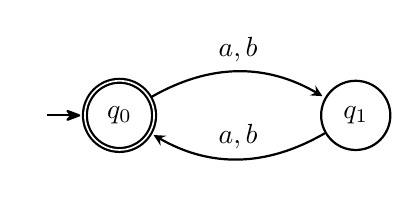
\begin{tikzpicture}[shorten >=1pt,node distance=3cm,on grid,>={Stealth[round]},thick]
		
		\node (q0) [state,initial, accepting, initial text = {}] {$q_0$};
		\node (q1) [state, right of = q0] {$q_1$};
		
		\path [-stealth, thick]
		(q0) edge [bend left] node [above] {$a,b$} (q1)
		(q1) edge [bend left] node [above] {$a,b$} (q0);
	\end{tikzpicture}

	$\delta:$
	\begin{table}[h]
		\centering
		\begin{tabular}{|c|c|c|}
			\hline
			Zustand & $a$ & $b$ \\
			\hline\hline
			$\emptyset$&$\emptyset$&$\emptyset$\\
			\hline
			$q_0$&\nm[$q_1$]&\nm[$q_1$]\\
			\hline
			$q_1$&\nm[$q_0$]&\nm[$q_0$]\\
			\hline
		\end{tabular}
	\end{table}
\end{center}
\qed
		\subsection*{(e) $E=\{w\mid w\in\{a,b\}^*,\#_a(w)-\#_b(w)\equiv0\mod3\}$}
			\begin{center}
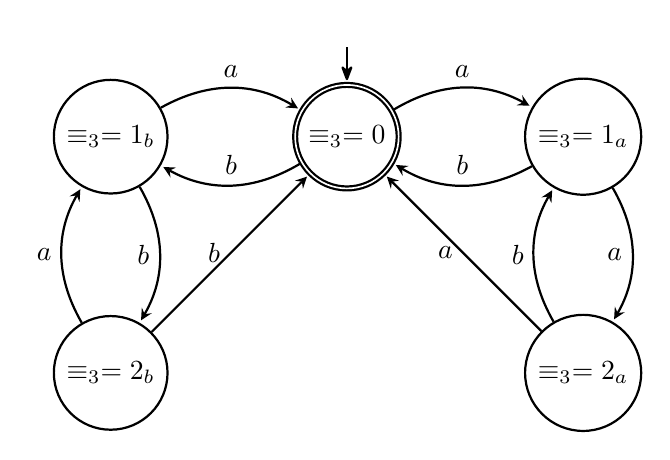
\begin{tikzpicture}[shorten >=1pt,node distance=3cm,on grid,>={Stealth[round]},thick]
	
	\node (s) [state, initial above, accepting, initial text = {}] {$\equiv_3=0$};
	\node (z1) [state, right of = s] {$\equiv_3=1_a$};
	\node (z2) [state, below of = z1] {$\equiv_3=2_a$};
	\node (z3) [state, left of = s] {$\equiv_3=1_b$};
	\node (z4) [state, below of = z3] {$\equiv_3=2_b$};
	
	\path [-stealth, thick]
	(s) edge [bend left] node [above] {$a$} (z1)
	(s) edge [bend left] node [above] {$b$} (z3)
	
	(z1) edge [bend left] node [left] {$a$} (z2)
	(z1) edge [bend left] node [above] {$b$} (s)
	
	(z2) edge node [left] {$a$} (s)
	(z2) edge [bend left] node [left] {$b$} (z1)
	
	(z3) edge [bend left] node [left] {$b$} (z4)
	(z3) edge [bend left] node [above] {$a$} (s)
	
	(z4) edge node [left] {$b$} (s)
	(z4) edge [bend left] node [left] {$a$} (z3);
\end{tikzpicture}

\newcommand{\q[1]}{$\{q_{#1}\}$}
\newcommand{\qq[1]}{$q_{#1}$}
\newcommand{\nz[2]}{$#1_#2$}
\newcommand{\nm[1]}{\{#1\}}
$\delta:$
\begin{table}[h]
	\centering
	\begin{tabular}{|c|c|c|}
		\hline
		Zustand & $a$ & $b$ \\
		\hline\hline
		$\emptyset$&$\emptyset$&$\emptyset$\\
		\hline
		$\equiv_3=0$&\nm[$\equiv_3=1_a$]&\nm[$\equiv_3=1_b$]\\
		\hline
		$\equiv_3=1_a$&\nm[$\equiv_3=2_a$]&\nm[$\equiv_3=0$]\\
		\hline
		$\equiv_3=2_a$&\nm[$\equiv_3=0$]&\nm[$\equiv_3=1_a$]\\
		\hline
		$\equiv_3=1_b$&\nm[$\equiv_3=0$]&\nm[$\equiv_3=2_b$]\\
		\hline
		$\equiv_3=2_b$&\nm[$\equiv_3=1_b$]&\nm[$\equiv_3=0$]\\
		\hline
	\end{tabular}
\end{table}
\end{center}
		\subsection*{(f) $F=\{0^{2^n}\mid n\in\mathbb{N}\}$ als Sprache über dem Alphabet $\{0\}$}
			\begin{proof}[Beweis]
	\begin{math}
		Ann:\;F\in REG\Rightarrow\;es\;gilt\;PL\Leftrightarrow\;Sei\;k\;Pumpingzahl:
	\end{math}
	\begin{align*}
		&Wähle\;x=\underbrace{0^{k-m}}_u\underbrace{0^m}_v\underbrace{0^k}_w,\mid x\mid\ge k;k\ge m\ge1\\\
		&Sei\;x=uvw\;eine\;geiegnete\;Zerlegung\;gemäß\;PL:\mid v\mid\ge1,\mid uv\mid\le k\\
		&\mid v\mid=k-m\ge 1\;und\;\mid uv\mid=k\le k\\
		&\overset{i=2}{\Longrightarrow}x=0^{k-2}0^{m^2}0^k=0^k0^m0^k=0^{2^k+m}\\
		&Betrachten\;wir\;die\;Exponenten:\\
		&2^k<2^k+m\le2^k+k,\quad da\;gilt:k\ge m\ge1\\
		&mit\;k<2^k\;folgt\\
		&2^k<2^k+m<2^{k+1}\\
		&\Rightarrow uv^2w\notin F\quad\lightning
	\end{align*}
\end{proof}
		\subsection*{(g) Die Menge aller Wörter $w$ über $\{0,1\}$, die als Binärzahl betrachtet durch 3 teilbar sind.}
			\newcommand{\nm[1]}{\{#1\}}
\begin{proof}[Beweis]
	\begin{math}
		Beh:
	\end{math}
	\begin{align*}
		&K_1=\[\lambda\]=\{w\in\{0,1\}^*\mid\text{ w ist als Binärzahl betrachtet durch 3 teilbar mit Rest 0}\}\\
		&K_2=\[1\]=\{w\in\{0,1\}^*\mid\text{ w ist als Binärzahl betrachtet durch 3 teilbar mit Rest 1}\}\\
		&K_3=\[10\]=\{w\in\{0,1\}^*\mid\text{ w ist als Binärzahl betrachtet durch 3 teilbar mit Rest 2}\}
	\end{align*}
	\begin{proof}[$K_1\cup K_2\cup K_3=\{a,b\}^*,K_i\;sind\;paarweise\;disjunkt$]
	\end{proof}
\end{proof}

\begin{center}
	$M=(\{0,1\},\{\equiv_3=0,\equiv_3=1,\equiv_3=2\},\delta,\{\equiv_3=0\},\{\equiv_3=0\})$\\
	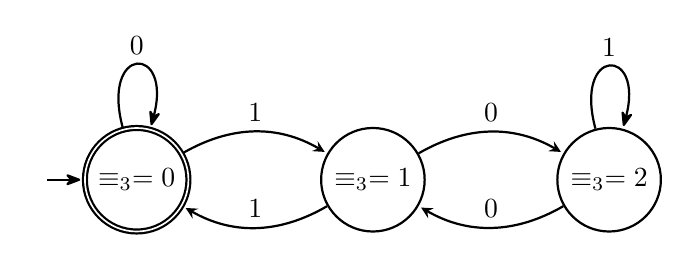
\begin{tikzpicture}[shorten >=1pt,node distance=3cm,on grid,>={Stealth[round]},thick]
		
		\node (q0) [state,initial, accepting, initial text = {}] {$\equiv_3=0$};
		\node (q1) [state, right of = q0] {$\equiv_3=1$};
		\node (q2) [state, right of = q1] {$\equiv_3=2$};
		
		\path [-stealth, thick]
		(q0) edge [loop above] node [above] {$0$} (q0)
		(q0) edge [bend left] node [above] {$1$} (q1)
		(q1) edge [bend left] node [above] {$1$} (q0)
		(q1) edge [bend left] node [above] {$0$} (q2)
		(q2) edge [bend left] node [above] {$0$} (q1)
		(q2) edge [loop above] node [above] {$1$} (q2);

	\end{tikzpicture}
	
	$\delta:$
	\begin{table}[h]
		\centering
		\begin{tabular}{|c|c|c|}
			\hline
			Zustand & $0$ & $1$ \\
			\hline\hline
			$\emptyset$&$\emptyset$&$\emptyset$\\
			\hline
			$\equiv_3=0$&\nm[$\equiv_3=0$]&\nm[$\equiv_3=1$]\\
			\hline
			$\equiv_3=1$&\nm[$\equiv_3=2$]&\nm[$\equiv_3=0$]\\
			\hline
			$\equiv_3=1$&\nm[$\equiv_3=1]$&\nm[$\equiv_3=2$]\\
			\hline
		\end{tabular}
	\end{table}
\end{center}
Wenn eine Zahl durch 3 Teilbar ist gibt es nur drei Möglichkeiten. Der Rest kann 0,1 oder 2 sein. Im DFA $M$ sind diese drei Zustände angegeben und in $\delta$ ihre Übergänge definiert. Man betrachtet die Wirkung der einzelnen Buchstaben auf das gesamte Wort und erkennt: wenn man in $\equiv_3=0$ ist ändert eine 0 nichts an der Teilbarkeit durch 3. Eine eins hingegen ehröht den Rest bei Division durch 3 auf 1. Deshalb landet man in $\equiv_3=1$. Wenn nun direkt eine 1 kommt wandert man wieder zurück, da dann $11_{bin}=3_{dez}$ angehängt wurde, was durch 3 mit Rest 0 teilbar ist. Fügt man hingegen eine 0 an und hat das Teilwort $10$ angehängt, so landet man in $\equiv_3=2$, da $10_{bin}=2_{dez}$. Von hier aus kann man mit einer 0 zurück, da $101_{bin}=4_dez\equiv_3=1$. Sollte man eine 1 lesen bleibt man solange im Zustand bis eine 0 kommt. Dies liegt daran, dass $1011_{bin}=11_{dez}\equiv_3=2,10111_{bin}=23\equiv_3=2,...$. $\Rightarrow G\in REG$.
		\subsection*{(h) $H=\{w\mid w\in\{a,b\}^*,w=w^R\}$ (Menge aller Palindorome über $\{a,b\}$)}
			\begin{proof}[Beweis]
	\begin{math}
		Ann:\;H\in REG\Rightarrow\;es\;gilt\;PL\Leftrightarrow\;Sei\;k\;Pumpingzahl:
	\end{math}
	\begin{align*}
		&Wähle\;x=\underbrace{a^{k-m}}_u\underbrace{a^m}_v\underbrace{b^ka^k}_w,\mid x\mid\ge k,m\ge1\\
		&Sei\;x=uvw\;eine\;geiegnete\;Zerlegung\;gemäß\;PL:\mid v\mid\ge1,\mid uv\mid\le k\\
		&\mid v\mid=m\ge1,\mid uv\mid = k\le k\\
		&\overset{i=0}{\Longrightarrow}x=a^{k-m}b^ka^k\notin H\quad\lightning
	\end{align*}
\end{proof}
		
	\section*{Aufgabe 2}
		Geben Sie für die Sprache $A=\{0^i1^j\mid i,j\ge0\}.$ Alle Äquivalenzklassen bezüglich der Relation $R_A$ an und beweisen Sie ihre Behauptung.
		\newcommand{\nc[4]}{#2&#3&#4\\\hline}
\begin{center}
	$M=(\{0,1\},\{0,0_1,0_2,0_3,1,2,2_1,2_2,2_3,2_4,2_5\},\delta,\{0_1\},\{0_2,1,2,2_1,2_4\})$
	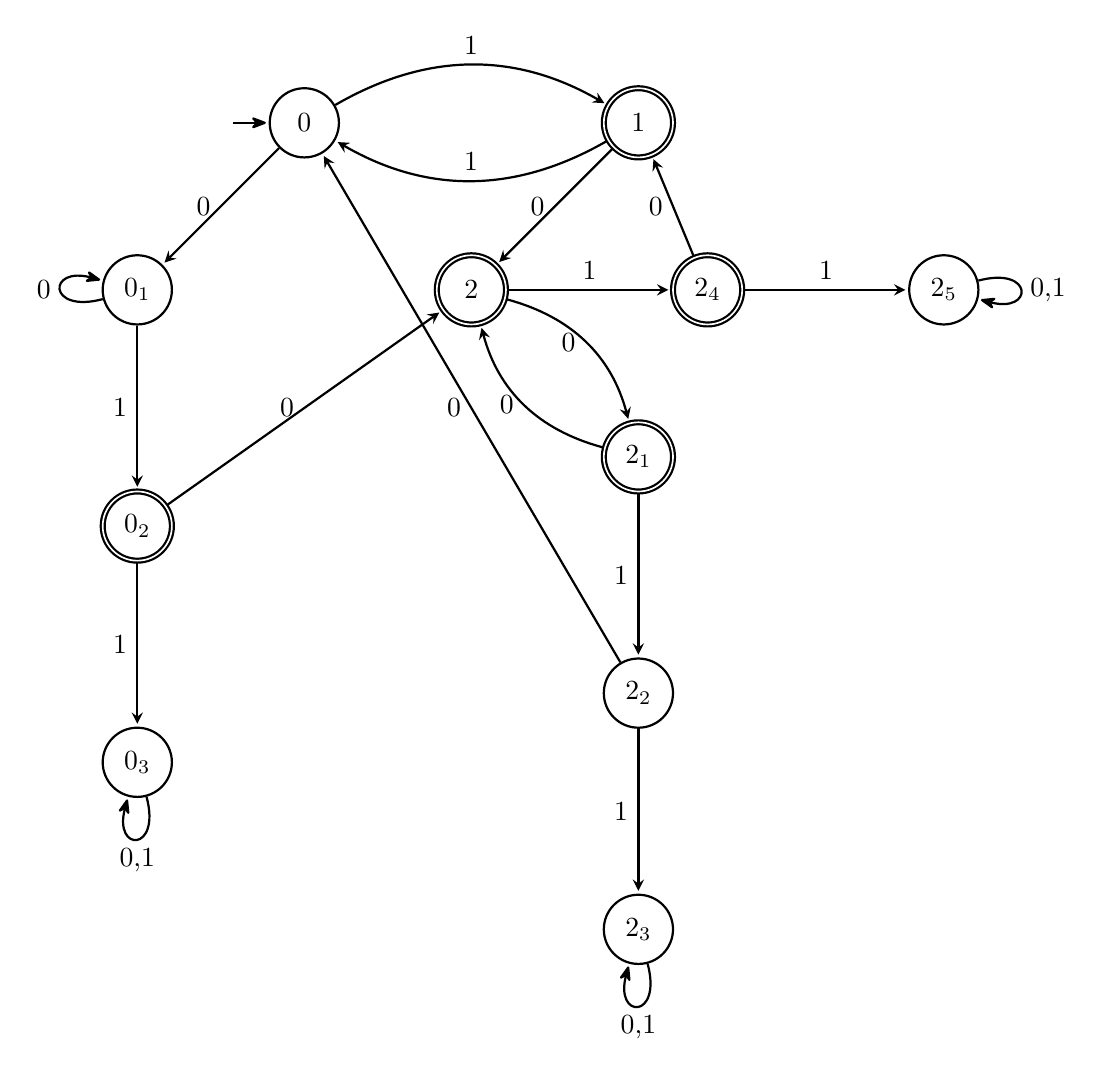
\begin{tikzpicture}[shorten >=1pt,node distance=3cm,on grid,>={Stealth[round]},thick]
		
		\node (q2) 
			[state, accepting] {2};
			\node (q21) 
				[state, accepting, below right of = q2] {$2_1$};
			\node (q22) 
				[state, below of = q21] {$2_2$};
			\node (q23) 
				[state, below of = q22] {$2_3$};
				
			\node (q24) 
				[state, accepting, right of = q2] {$2_4$};
			\node (q25) 
				[state, right of = q24] {$2_5$};
			
			
		\node (q0) 
			[state, initial, initial text = {}, above left of = q2] {0};
			\node (q01) 
				[state, below left of = q0] {$0_1$};
			\node (q02) 
				[state, accepting, below of = q01] {$0_2$};
			\node (q03) 
				[state, below of = q02] {$0_3$};
			
			
		\node (q1) 
			[state, accepting, above right of = q2] {1};
			
		
		
		\path [-stealth, thick]
		%(q0) edge [loop above] node [above] {$0$} (q0)
		(q0) edge [bend left] node [above] {1} (q1)
		(q0) edge node [left] {0} (q01)
		(q01) edge node [left] {1} (q02)
		(q02) edge node [left] {1} (q03)
		(q03) edge [loop below] node [below] {0,1} (q03)
		
		(q1) edge [bend left] node [above] {1} (q0)
		(q1) edge node [left] {0} (q2)
		
		(q2) edge [bend left] node [left] {0} (q21)
		(q21) edge [bend left] node [left] {0} (q2)
		(q21) edge node [left] {1} (q22)
		(q22) edge node [left] {1} (q23)
		(q22) edge node [left] {0} (q0)
		
		(q2) edge node [above] {1} (q24)
		(q24) edge node [above] {1} (q25)
		
		(q01) edge [loop left] node [left] {0} (q01)
		(q23) edge [loop below] node [below] {0,1} (q23)
		(q24) edge node [left] {0} (q1)
		(q25) edge [loop right] node [right] {0,1} (q25)
		(q02) edge node [left] {0} (q2)
		;
	\end{tikzpicture}
	
	$\delta:$
	\begin{table}[h]
		\centering
		\begin{tabular}{|c|c|c|}
			\hline
			Zustand & $0$ & $1$ \\
			\hline\hline
			\nc{$0$}{$0_1$}{$1$}
			\nc{$0_1$}{$0_1$}{$0_2$}
			\nc{$0_2$}{$2$}{$0_3$}
			\nc{$0_3$}{$0_3$}{$0_3$}
			\nc{$1$}{$2$}{$0$}
			\nc{$2$}{$2_1$}{$2_4$}
			\nc{$2_1$}{$2$}{$2_2$}
			\nc{$2_2$}{$0$}{$2_3$}
			\nc{$2_3$}{$2_3$}{$2_3$}
			\nc{$2_4$}{$1$}{$2_5$}
			\nc{$2_5$}{$2_5$}{$2_5$}
		\end{tabular}
	\end{table}
\end{center}
Der Automat ist folgendermaßen entstanden: Ich habe den Automaten der letzten Übungsserie genommen in dem beschrieben wird wann eine binär Zahl durch 3 teilbar ist:
\begin{center}
	$M_2=(\{0,1\},\{\equiv_3=0,\equiv_3=1,\equiv_3=2\},\delta_2,\{\equiv_3=0\},\{\equiv_3=0\})$\\
	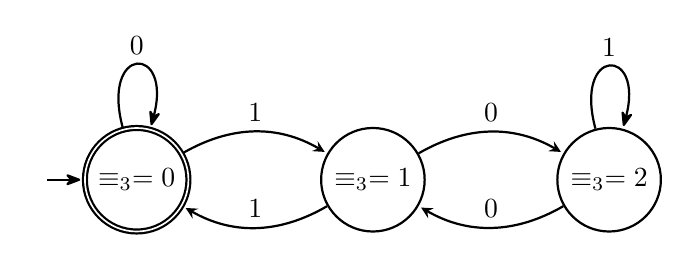
\begin{tikzpicture}[shorten >=1pt,node distance=3cm,on grid,>={Stealth[round]},thick]
		
		\node (q0) [state,initial, accepting, initial text = {}] {$\equiv_3=0$};
		\node (q1) [state, right of = q0] {$\equiv_3=1$};
		\node (q2) [state, right of = q1] {$\equiv_3=2$};
		
		\path [-stealth, thick]
		(q0) edge [loop above] node [above] {$0$} (q0)
		(q0) edge [bend left] node [above] {$1$} (q1)
		(q1) edge [bend left] node [above] {$1$} (q0)
		(q1) edge [bend left] node [above] {$0$} (q2)
		(q2) edge [bend left] node [above] {$0$} (q1)
		(q2) edge [loop above] node [above] {$1$} (q2);
		
	\end{tikzpicture}
	
	$\delta_2:$
	\begin{table}[h]
		\centering
		\begin{tabular}{|c|c|c|}
			\hline
			Zustand & $0$ & $1$ \\
			\hline\hline
			$\emptyset$&$\emptyset$&$\emptyset$\\
			\hline
			$\equiv_3=0$&\nm[$\equiv_3=0$]&\nm[$\equiv_3=1$]\\
			\hline
			$\equiv_3=1$&\nm[$\equiv_3=2$]&\nm[$\equiv_3=0$]\\
			\hline
			$\equiv_3=1$&\nm[$\equiv_3=1]$&\nm[$\equiv_3=2$]\\
			\hline
		\end{tabular}
	\end{table}
\end{center}
Von hier aus habe ich dann alle Fälle betrachtet in denen eine $0$ gelesen wird und habe diese dann zu einem dedizierten Zustand weitergeleitet. In jedem dieser Fälle habe ich dann betrachtet wie sich sowohl die Nicht-Teilbarkeit durch 3 verhält, als auch ob ein neuer Zustand benötigt wird um das Teilwort $011$ zu kapseln. Dieser Automat kann prinzipiell jedes Wort lesen. Wenn jedoch eine Sequenz $011$ auftritt, egal wo man sich vorher befunden hat, so  endet man in $0_3\lor2_3\lor2_5$. Somit ist wenn dieses Teilwort aufgetreten ist es nicht mehr möglich akzeptiert zu werden. In allen anderen fällen ist es möglich ein Wort zu lesen, dass akzeptiert wird, hierfür muss jedoch die Nicht-Teilbarkeit durch 3 gegeben sein. Dieses habe ich mittels dem Automaten der Übungsserie 4 abgeleitet. Jeder Zustand im Automaten besitzt neben der Information welche Zahlen vor ihm gelesen wurden auch die Information ob er durch 3 Teilbar ist oder nicht. Diese Informationen verteilen sich wie folgt: $0,0_1,2_2$ sind durch 3 teilbar. $1,0_2,2_1$ sind durch 3 Rest 1 teilbar und somit zu akzeptieren. Und $2,2_4$ sind durch 3 Rest 2 teilbar und folglich auch zu akzeptieren. 
	
\endgroup\end{document}